\documentclass{article}

\usepackage{siunitx} % Provides the \SI{}{} and \si{} command for typesetting SI units
\usepackage{graphicx} % Required for the inclusion of images
\usepackage{amsmath}
\usepackage{amsfonts}
\usepackage[T1]{fontenc}
\usepackage[utf8]{inputenc}
\usepackage[margin=0.75in]{geometry}
\usepackage{isotope}
\usepackage{wrapfig}
\setlength\parindent{0pt}

\title{Investigating hyperfine structure properties of Caesium and measuring Earth's magnetic flux density using optical pumping.} % Title

\newcommand{\Z}{\mathbb{Z}}

\author{Joshua Porter} % Author name

\date{} % Date for the report
\pagenumbering{gobble}
\begin{document}
\maketitle
\abstract{Determining the Hyperfine Landé g-factor of the $6^2S_{1/2}$ $F=4$ sub-state.}


\section{Aims of the experiment}
To create a plot of resonant frequency of the transition between two states as a function of Helmholtz coil current and extract information by fitting a function to the data. Alter the set-up to detect and record Rabi oscillations and determine what information can be extracted from the oscilloscope recording of the oscillations.
\section{Background}
Optical pumping is the technique by which level populations of a system can be manipulated such that a single magnetic sub-level can be fully and (semi-)inescapably populated. The most famous use of this is to achieve population inversion for producing laser light.

\begin{wrapfigure}{h}{0.3\linewidth}
	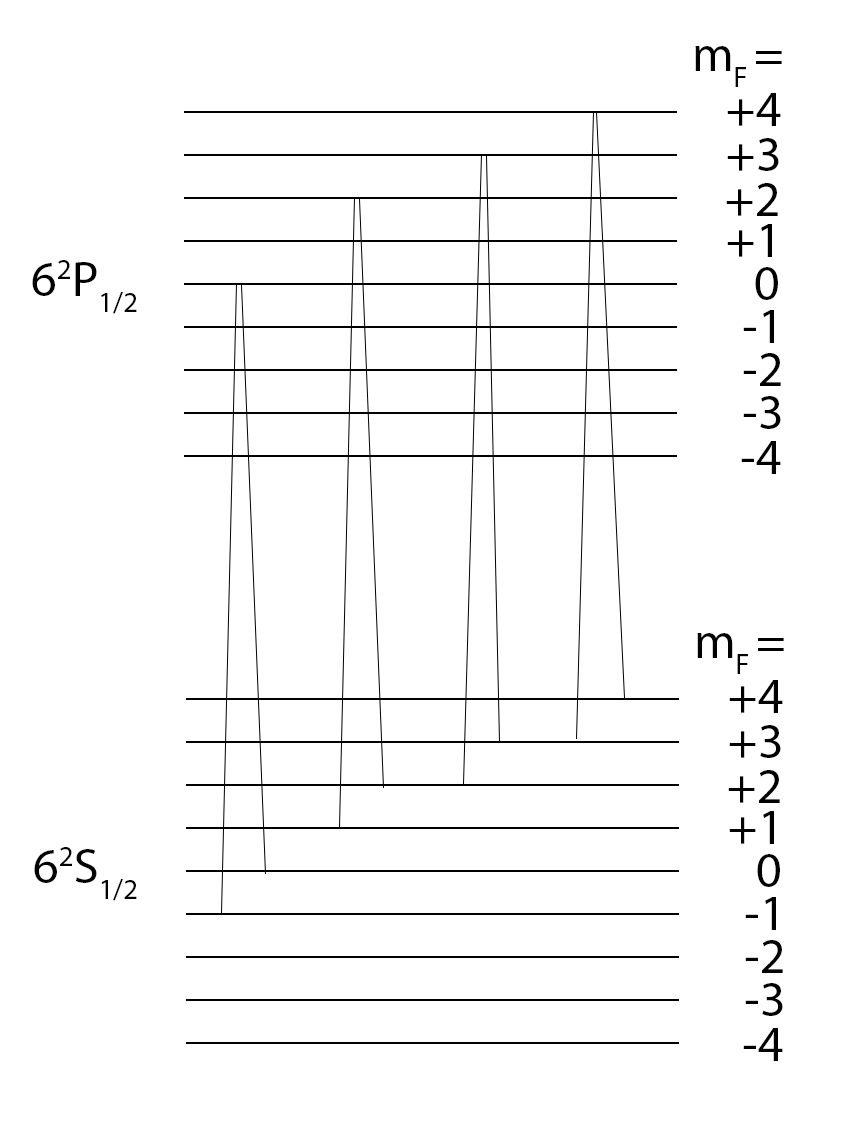
\includegraphics[width=0.3\textwidth]{figure2}
	\caption{Unshielded background spectrum.}
	\label{}
\end{wrapfigure}%

This is achieved by designing a pumping mechanism with selection rules that create a 'terminal' energy sub-state to which all of a system's population moves towards. Take the example of a system with an upper and lower level both of which have total angular momentum $F=4$. These can be split into magnetic sub-states $m_F \in \Z : m_F \in [-F, F]$. Initially the populations can be described by a Boltzmann distribution where the majority of the population lays in the lowest $m_F$ levels. Circularly polarized with the selection rule for absorption $\Delta m_F=1$ is then incident on the system. Electrons in levels $m_F=-4, -3,...,3$ will be excited to the equivalent $m_F+1$ level in the excited level before decaying to the ground state $m_F$ levels allowed by the selection rule $\Delta m_F=-1,0,+1$. However, if the ground state sub-level it de-excites into is $m_F=4$ then there is no $m_F+1$ level in the excited state to move into, neither is there a lower energy state to de-excite further into. Until new de-excitation channels are introduced the electron is effectively trapped in this state.
\section{Saturation spectroscopy apparatus}

\section{Analysis}

\section{Results}
\begin{table}[h]
	\centering
	\ {\def\arraystretch{1.2}\tabcolsep=20pt\
\begin{tabular}{ccc}
	\hline\ Parameter & Value \\ 
	\hline
	Earth's magnetic flux density & $0.4858 \pm 0.017$ G \\ 
	NOAA Earth's magnetic flux density & $0.4859 \pm 0.0015$ G \\ 
	$\sigma$ difference & 0.0054 \\
	\hline
	Landé g-factor & $0.2484 \pm 0.0086$ & \\
	Calculated Landé g-factor & $~0.24994$ & \\
	$\sigma$ difference & 0.0054 \\
	\hline
\end{tabular}%
\ }
\end{table}%

\begin{figure}[h!]
\begin{center}
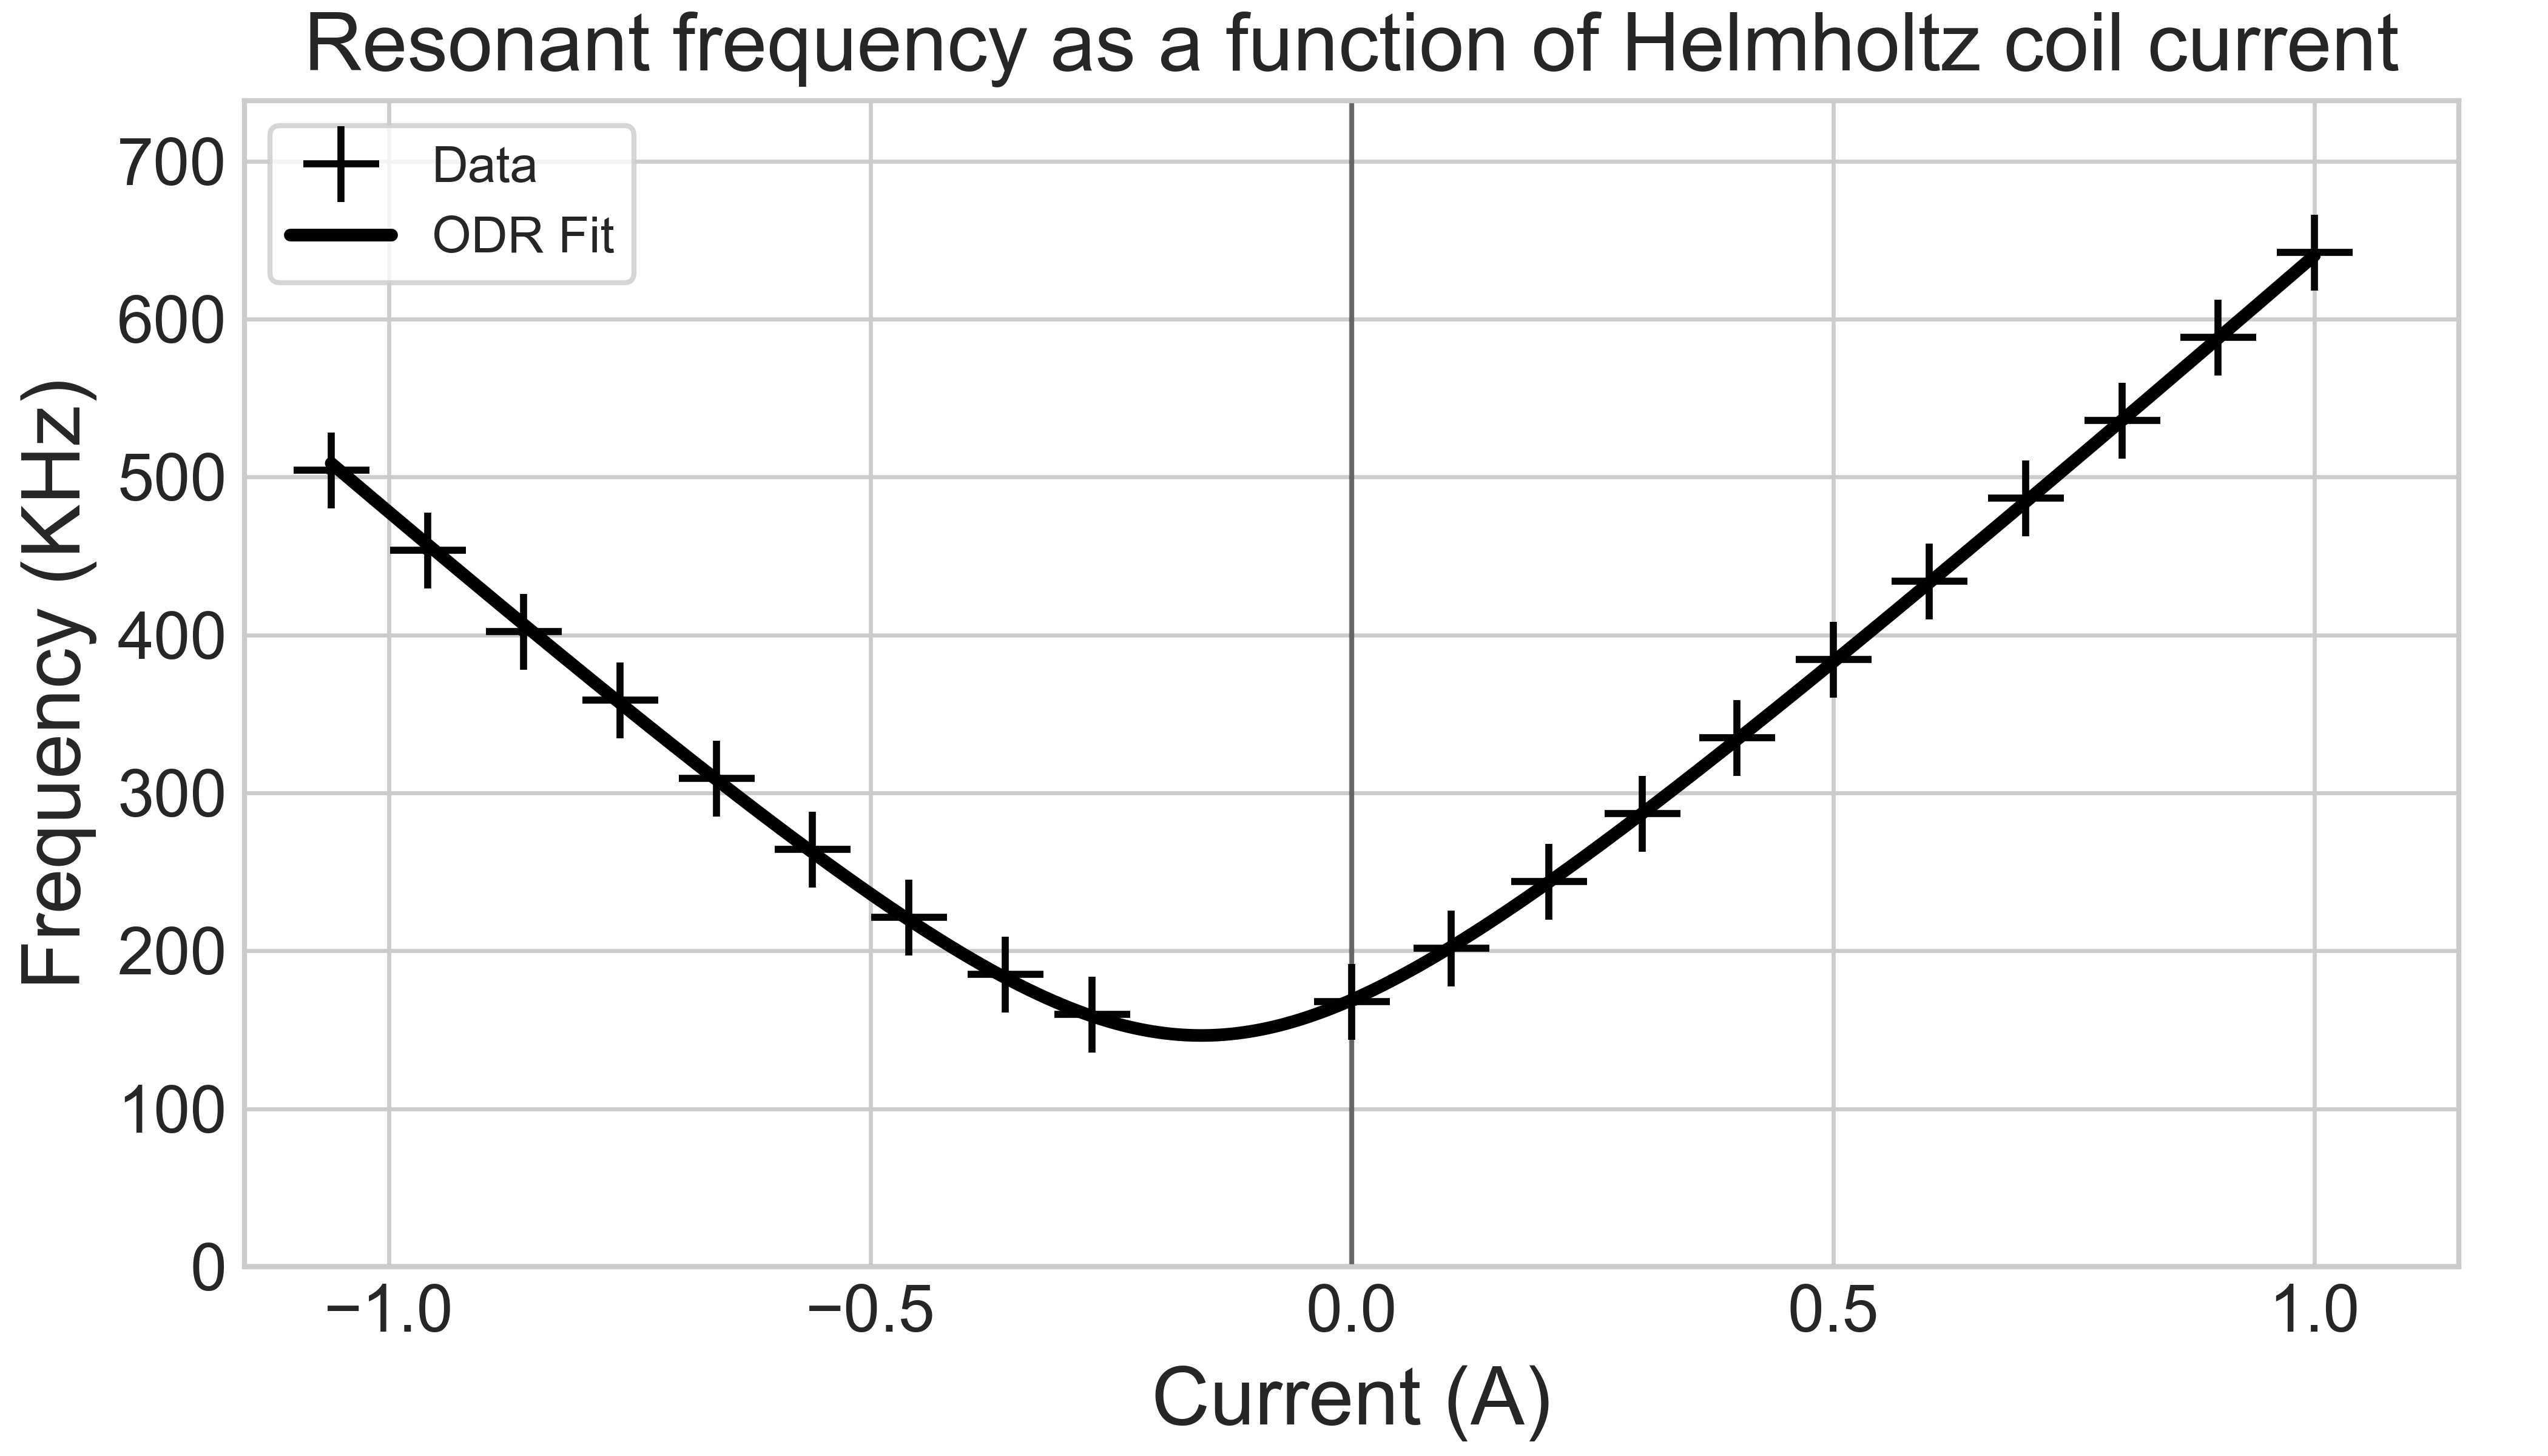
\includegraphics[width=0.65\textwidth]{figure1}
\caption{}
\end{center}%
\end{figure}%


\section{Discussion}

\section{Conclusion}

\end{document}